\section{System Framework}



%===============================================
\begin{figure}[t]
	\centering
	% \vspace{-4mm}
	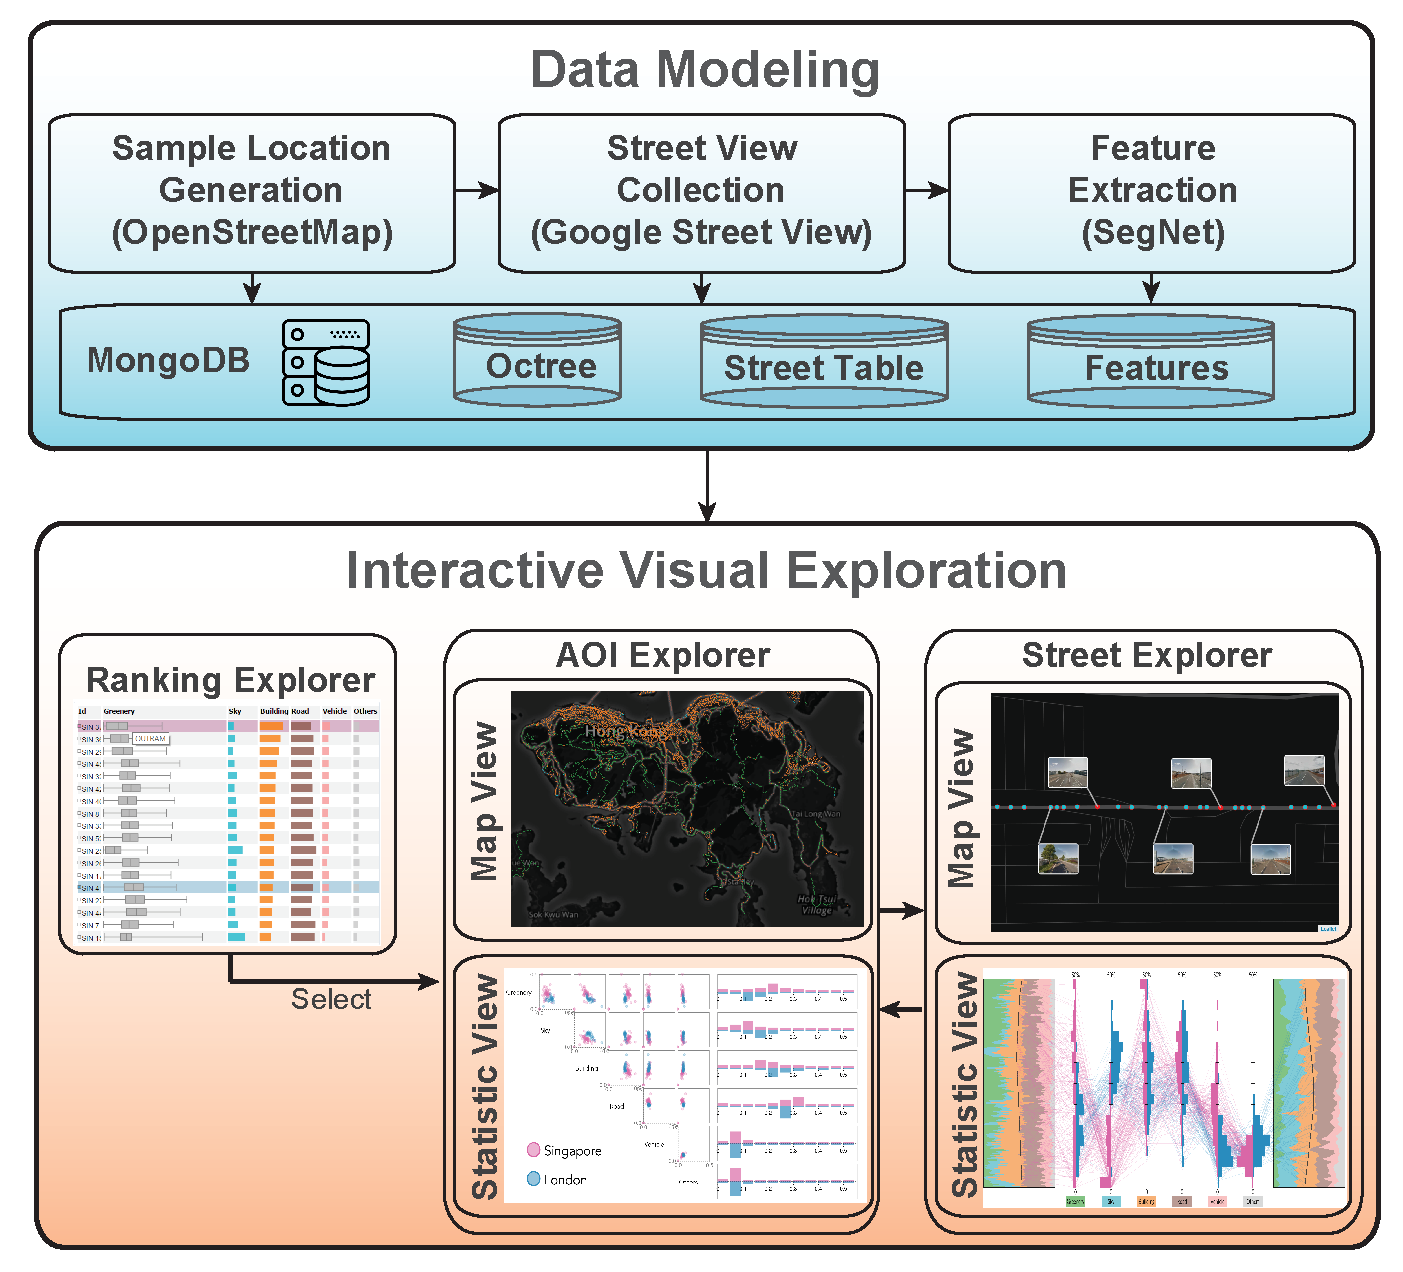
\includegraphics[width=0.9\columnwidth]{figures/streetvizor/fig2_framework/framework.pdf}
	\vspace{-5mm}
	\caption{Overview of StreetVizor workflow. Our system consists of two phases: data modeling and interactive visual exploration.}
	\label{fig:sys_overview}
	\vspace{-6mm}
\end{figure}

StreetVizor is a web-based application comprising two major phases, as illustrated in Fig.~\ref{fig:sys_overview}.
In the data modeling phase, our system automatically collects hundreds of thousands of GSV images at sampling positions in each city generated from OpenStreetMap (OSM) (Section~\ref{ssec:data_collection}).
Then, we classify the pixels of the collected images into 12 classes using SegNet, and extract the desired feature metric from the classification results (Section~\ref{ssec:feature}).
Data collection and preprocessing are conducted offline on a high-performance workstation with 12 core 3.40 GHz Intel Core i7-6800K CPU and a GeForce GTX 1080 graphics card.
Though enabled with GPU acceleration, the computation still takes several to 20 hours to preprocess images from each city.
Then, we construct data structures, including an octree and a lookup table, to facilitate visual exploration, such as spatial query and filtering (Section~\ref{ssec:query}).
The datasets are stored in a back-end MongoDB server with 2.4 GHz Intel Xeon E5-2620 CPU and 64 GB memory.

The interactive visual exploration phase consists of two stages:
1) Our system provides users with a Ranking Explorer that ranks and compares multiple AOIs/streets based on human-scale urban forms.
Users can narrow down exploration by selecting two AOIs/streets for detailed comparison. 
2) If two AOIs are selected, the system will present an AOI Explorer that compares the differences in human-scale urban forms in two AOIs at city- and region-scales.
The AOI Explorer is composed of CMVs, including two juxtaposition map views for spatial exploration and a superposition statistic view for comparing various quantitative measurements, such as feature correlations and diversities.
Users can further navigate down to select two streets, and our system will provide Street Explorer, which presents the fine details of human-scale urban forms at street-level.
In Street Explorer, we present map views that show the geographical information and representative images of two streets.
We also develop a novel PCP enhanced with themeriver along street layouts, allowing users to compare multivariate features and reveal feature distributions along the two streets.
The visualization modules are implemented in D3.js and Three.js for different rendering requirements, and they are integrated using Vue.js.

\if 0

. Whole system framework is shown in the figure.2.
The whole system pipeline starts from the data process models. Data process model will collect and analysis Google street view images, mark them with gps tags and generate the human-scale feature vector automatically . The output of the human-scale features with gps information will be stored by mongodb, a nosql database, the correponding geographical index will be generated to improve query speed. Based on mongodb, we build web server with Python/Flask, and Frontend system with Vuejs. The viusalization module are implemented by D3 and Three.js for different render requirement.

The visualization module consists of tow major view: navigation view and analysis view. Navigation view provides high level overview of the human-scale feature distribution as well as many flexible query methods. Users can navigate from different level in the navigation view, to find the analysis target or narrow down to a smaller scope, e.g. a smaller subset of streets or regions. For the selected units, users can conduct an find granularity analysis...

\fi